% Options for packages loaded elsewhere
\PassOptionsToPackage{unicode}{hyperref}
\PassOptionsToPackage{hyphens}{url}
\PassOptionsToPackage{dvipsnames,svgnames,x11names}{xcolor}
%
\documentclass[
]{article}

\usepackage{amsmath,amssymb}
\usepackage{iftex}
\ifPDFTeX
  \usepackage[T1]{fontenc}
  \usepackage[utf8]{inputenc}
  \usepackage{textcomp} % provide euro and other symbols
\else % if luatex or xetex
  \usepackage{unicode-math}
  \defaultfontfeatures{Scale=MatchLowercase}
  \defaultfontfeatures[\rmfamily]{Ligatures=TeX,Scale=1}
\fi
\usepackage{lmodern}
\ifPDFTeX\else  
    % xetex/luatex font selection
\fi
% Use upquote if available, for straight quotes in verbatim environments
\IfFileExists{upquote.sty}{\usepackage{upquote}}{}
\IfFileExists{microtype.sty}{% use microtype if available
  \usepackage[]{microtype}
  \UseMicrotypeSet[protrusion]{basicmath} % disable protrusion for tt fonts
}{}
\makeatletter
\@ifundefined{KOMAClassName}{% if non-KOMA class
  \IfFileExists{parskip.sty}{%
    \usepackage{parskip}
  }{% else
    \setlength{\parindent}{0pt}
    \setlength{\parskip}{6pt plus 2pt minus 1pt}}
}{% if KOMA class
  \KOMAoptions{parskip=half}}
\makeatother
\usepackage{xcolor}
\setlength{\emergencystretch}{3em} % prevent overfull lines
\setcounter{secnumdepth}{5}
% Make \paragraph and \subparagraph free-standing
\ifx\paragraph\undefined\else
  \let\oldparagraph\paragraph
  \renewcommand{\paragraph}[1]{\oldparagraph{#1}\mbox{}}
\fi
\ifx\subparagraph\undefined\else
  \let\oldsubparagraph\subparagraph
  \renewcommand{\subparagraph}[1]{\oldsubparagraph{#1}\mbox{}}
\fi


\providecommand{\tightlist}{%
  \setlength{\itemsep}{0pt}\setlength{\parskip}{0pt}}\usepackage{longtable,booktabs,array}
\usepackage{calc} % for calculating minipage widths
% Correct order of tables after \paragraph or \subparagraph
\usepackage{etoolbox}
\makeatletter
\patchcmd\longtable{\par}{\if@noskipsec\mbox{}\fi\par}{}{}
\makeatother
% Allow footnotes in longtable head/foot
\IfFileExists{footnotehyper.sty}{\usepackage{footnotehyper}}{\usepackage{footnote}}
\makesavenoteenv{longtable}
\usepackage{graphicx}
\makeatletter
\def\maxwidth{\ifdim\Gin@nat@width>\linewidth\linewidth\else\Gin@nat@width\fi}
\def\maxheight{\ifdim\Gin@nat@height>\textheight\textheight\else\Gin@nat@height\fi}
\makeatother
% Scale images if necessary, so that they will not overflow the page
% margins by default, and it is still possible to overwrite the defaults
% using explicit options in \includegraphics[width, height, ...]{}
\setkeys{Gin}{width=\maxwidth,height=\maxheight,keepaspectratio}
% Set default figure placement to htbp
\makeatletter
\def\fps@figure{htbp}
\makeatother

% \usepackage[figon, printfigures]{figcaps}
\usepackage{booktabs}
\usepackage{longtable}
\usepackage{array}
\usepackage{multirow}
\usepackage{wrapfig}
\usepackage{float}
\usepackage{colortbl}
\usepackage{pdflscape}
\usepackage{tabu}
\usepackage{threeparttable}
\usepackage{threeparttablex}
\usepackage[normalem]{ulem}
\usepackage{makecell}
\usepackage{xcolor}
\makeatletter
\@ifpackageloaded{caption}{}{\usepackage{caption}}
\AtBeginDocument{%
\ifdefined\contentsname
  \renewcommand*\contentsname{Table of contents}
\else
  \newcommand\contentsname{Table of contents}
\fi
\ifdefined\listfigurename
  \renewcommand*\listfigurename{List of Figures}
\else
  \newcommand\listfigurename{List of Figures}
\fi
\ifdefined\listtablename
  \renewcommand*\listtablename{List of Tables}
\else
  \newcommand\listtablename{List of Tables}
\fi
\ifdefined\figurename
  \renewcommand*\figurename{Figure}
\else
  \newcommand\figurename{Figure}
\fi
\ifdefined\tablename
  \renewcommand*\tablename{Table}
\else
  \newcommand\tablename{Table}
\fi
}
\@ifpackageloaded{float}{}{\usepackage{float}}
\floatstyle{ruled}
\@ifundefined{c@chapter}{\newfloat{codelisting}{h}{lop}}{\newfloat{codelisting}{h}{lop}[chapter]}
\floatname{codelisting}{Listing}
\newcommand*\listoflistings{\listof{codelisting}{List of Listings}}
\makeatother
\makeatletter
\makeatother
\makeatletter
\@ifpackageloaded{caption}{}{\usepackage{caption}}
\@ifpackageloaded{subcaption}{}{\usepackage{subcaption}}
\makeatother
\ifLuaTeX
  \usepackage{selnolig}  % disable illegal ligatures
\fi
\usepackage{bookmark}

\IfFileExists{xurl.sty}{\usepackage{xurl}}{} % add URL line breaks if available
\urlstyle{same} % disable monospaced font for URLs
\hypersetup{
  pdftitle={Simulations Report},
  pdfauthor={Hans Martinez},
  colorlinks=true,
  linkcolor={blue},
  filecolor={Maroon},
  citecolor={Blue},
  urlcolor={Blue},
  pdfcreator={LaTeX via pandoc}}

\title{Simulations Report}
\author{Hans Martinez}
\date{2025-06-16}

\begin{document}
\maketitle

\section{The Data Generating Process}\label{the-data-generating-process}

The DGP process used in these simulations is as follows.

\[
\begin{aligned}
    y_l, x_l &\sim (1-\rho)\epsilon_l +\rho \eta_l \\
    \epsilon_l &\sim N(0,1) \\
    \eta_l &\sim \mathcal{G}(\theta)
\end{aligned}
\]

\((y_l,x_l,\epsilon_l,\eta_l)\) are associated with observed spatial
location \(s_l \in \mathbb{R}^2\). \(\epsilon\) is a white noise
independent of \(s_l\). \(\eta\) is generated by a Gaussian process with
covariance function
\(cov(s_l,s_{l'})=\exp(-\theta^{-1}||s_l-s_{l'}||)\). The parameter
\(\rho\in[0,1)\) controls the spatial correlation of observations.

\section{Simulations}\label{simulations}

In the simulations, the regression model is

\[
    y_l=\beta x_l + u_l
\]

because \(y_l\) and \(x_l\) are independent draws from the same DGP, the
true parameter is \(\beta=0\). The parameter of the gaussian process was
set as \(\theta=\sqrt{2}/10\). \textbf{500} observations were drawn of
each variable \((y_l,x_l,s_l)\). Locations \(s_l\) were drawn from the
uniform Poisson process inside the unit square, two for each
observation. The rejection frequencies are the fraction of the
\textbf{1000} simulations that the the null hypothesis \(H_0: \beta=0\)
was rejected in favor of the alternative \(H_1: \beta\not=0\).

\section{Spatial vs.~Time Series correlation}\label{sec-ar1}

For reference, when \(\rho=1\), the average of the elements of the
variance-covariance matrix resulting from the covariance function
\(cov(s_l,s_{l'})=\exp(-\theta^{-1}||s_l-s_{l'}||)\) with
\(\theta=\sqrt{2}/10\) is 0.0839. This value is approximately equivalent
to an AR(1) process with a slope of \textasciitilde0.96.

The following table shows the average of the elements of the
variance-covariance matrix of an AR(1) process with different values of
autocorrelation, \(\delta\). That is, for a value of \(\delta\) and
\(T\) observations, the var-cov matrix will look like the following:

\[
    V = \begin{pmatrix}
    1 & \delta & \delta^2 & \cdots & \delta^{T-1} \\
    \delta & 1 & \delta & \cdots & \delta^{T-2} \\
    \delta^2 & \delta & 1 & \cdots & \delta^{T-3} \\
    \vdots & \vdots & \vdots & \ddots & \vdots \\
    \delta^{T-1} & \delta^{T-2} & \delta^{T-3} & \cdots & 1
    \end{pmatrix}
\]

\begin{longtable}[]{@{}ll@{}}
\toprule\noalign{}
\(\delta\) & Average \\
\midrule\noalign{}
\endhead
\bottomrule\noalign{}
\endlastfoot
0.94 & 0.0626 \\
0.95 & 0.0750 \\
0.96 & 0.0932 \\
0.97 & 0.1227 \\
\end{longtable}

\section{Results}\label{results}

\subsection{Triangle B-Splines}\label{triangle-b-splines}

Table~\ref{tbl-HAC-8x8-u-slope-tri} displays the rejection frequencies
of testing the null hypothesis that the slope is statistically different
from the true value, zero, at the 5 percent significance level for
different levels of spatial correlation. The table compares using the
8x8 B Splines on locations for prewhitening. Different variance
estimators are employed.

\begin{table}

\caption{\label{tbl-HAC-8x8-u-slope-tri}Rejection frequencies testing
the null hypothesis that the slope is statically different from the true
value, zero, at the 5\% significance level for different values of
spatial correlation (\(\rho\)), using the \textbf{gaussian} kernel HAC
variance estimator for the standard error for different cutoff lengths
with and without 8x8 \textbf{triangle} B-splines. 1000 simulations. 500
points. Column \emph{Corr} shows the theoretical correlation at distance
\(h=0.1\), \(Corr=\rho*\exp(-\frac{1}{\sqrt{2}})\). Cutoff lengths are
equal to \(2\sigma\) in the gaussian kernel.}

\centering{

\begin{tabular}{rrrrrrrrrr}
\toprule
\multicolumn{2}{c}{ } & \multicolumn{4}{c}{No Splines} & \multicolumn{4}{c}{Triangle Splines} \\
\cmidrule(l{3pt}r{3pt}){3-6} \cmidrule(l{3pt}r{3pt}){7-10}
\multicolumn{2}{c}{ } & \multicolumn{3}{c}{HAC} & \multicolumn{1}{c}{ } & \multicolumn{3}{c}{HAC} \\
\cmidrule(l{3pt}r{3pt}){3-5} \cmidrule(l{3pt}r{3pt}){7-9}
$\rho$ & Corr & .05 & .10 & .15 & HR & .05 & .10 & .15 & HR \\
\midrule
0.0 & 0.00 & 0.06 & 0.06 & 0.06 & 0.06 & 0.06 & 0.06 & 0.06 & 0.06\\
0.1 & 0.05 & 0.07 & 0.07 & 0.07 & 0.08 & 0.05 & 0.05 & 0.05 & 0.06\\
0.2 & 0.10 & 0.13 & 0.12 & 0.11 & 0.14 & 0.05 & 0.05 & 0.05 & 0.06\\
0.3 & 0.15 & 0.16 & 0.13 & 0.12 & 0.18 & 0.04 & 0.04 & 0.05 & 0.04\\
0.4 & 0.20 & 0.24 & 0.19 & 0.16 & 0.27 & 0.06 & 0.05 & 0.06 & 0.06\\
\addlinespace
0.5 & 0.25 & 0.26 & 0.21 & 0.16 & 0.32 & 0.06 & 0.06 & 0.06 & 0.06\\
0.6 & 0.30 & 0.30 & 0.22 & 0.17 & 0.37 & 0.06 & 0.06 & 0.06 & 0.07\\
0.7 & 0.35 & 0.37 & 0.28 & 0.22 & 0.48 & 0.07 & 0.07 & 0.07 & 0.08\\
0.8 & 0.39 & 0.39 & 0.28 & 0.23 & 0.52 & 0.09 & 0.07 & 0.07 & 0.09\\
0.9 & 0.44 & 0.43 & 0.31 & 0.24 & 0.57 & 0.09 & 0.08 & 0.07 & 0.11\\
\addlinespace
1.0 & 0.49 & 0.42 & 0.30 & 0.22 & 0.59 & 0.13 & 0.11 & 0.10 & 0.18\\
\bottomrule
\end{tabular}

}

\end{table}%

\begin{table}

\caption{\label{tbl-HAC-8x8-u-ci-unif-bs-morgan}Confidence Interval
length of different HAC variance estimators of the standard error with
an 8x8 \textbf{triangular} B-splines. 1000 simulations. \textbf{500}
points. Column \emph{Corr} shows the theoretical correlation at distance
\(h=0.1\), \(corr=\rho*\exp(-\frac{1}{\sqrt{2}})\).}

\centering{

\begin{tabular}{rrrrrr}
\toprule
\multicolumn{2}{c}{ } & \multicolumn{3}{c}{HAC} \\
\cmidrule(l{3pt}r{3pt}){3-5}
$\rho$ & Corr & .05 & .10 & .15 & HR\\
\midrule
0.0 & 0.00 & 0.19 & 0.19 & 0.19 & 0.19\\
0.1 & 0.05 & 0.19 & 0.19 & 0.19 & 0.19\\
0.2 & 0.10 & 0.19 & 0.19 & 0.19 & 0.19\\
0.3 & 0.15 & 0.19 & 0.19 & 0.19 & 0.19\\
0.4 & 0.20 & 0.19 & 0.19 & 0.19 & 0.19\\
\addlinespace
0.5 & 0.25 & 0.19 & 0.19 & 0.19 & 0.19\\
0.6 & 0.30 & 0.19 & 0.19 & 0.19 & 0.19\\
0.7 & 0.35 & 0.19 & 0.19 & 0.20 & 0.19\\
0.8 & 0.39 & 0.20 & 0.20 & 0.20 & 0.19\\
0.9 & 0.44 & 0.20 & 0.21 & 0.22 & 0.19\\
\addlinespace
1.0 & 0.49 & 0.22 & 0.23 & 0.24 & 0.19\\
\bottomrule
\end{tabular}

}

\end{table}%

\subsection{PCs}\label{pcs}

In this section, instead of using the whole 8x8 B-Splines, the first
\(n\) ordered principal components of the B-Splines are used. In each
iteration, \(n\) is choosen to minimize the absolute difference between
the nearest neighbour correlation and 5\%. The principal components are
sorted in decreasing order by their variance.

Table~\ref{tbl-pc} displays the results of the simulations.

\begin{table}

\caption{\label{tbl-pc}Rejection frequencies testing the null hypothesis
that the slope is statically different from the true value, zero, at the
5\% significance level for different values of spatial correlation
(\(\rho\)), using the \textbf{gaussian} kernel HAC variance estimator
for the standard error for different cutoff lengths. The table compares
estimates of prewhitening by including the number of principal
components of the 8x8 \textbf{triangle} B-splines that minimizes the
nearest neighbour correlation to 5\%. 1000 simulations. 500 points.
Column \emph{Corr} shows the theoretical correlation at distance
\(h=0.1\), \(Corr=\rho*\exp(-\frac{1}{\sqrt{2}})\). Cutoff lengths are
equal to \(2\sigma\) in the gaussian kernel. NN is the nearest neighbour
correlation after prewhitening with the B-Splines. PCs is the average
number of principal components used in simulations.}

\centering{

\begin{tabular}{rrrrrrrrrrrr}
\toprule
\multicolumn{2}{c}{ } & \multicolumn{4}{c}{No Splines} & \multicolumn{6}{c}{Triangle Splines} \\
\cmidrule(l{3pt}r{3pt}){3-6} \cmidrule(l{3pt}r{3pt}){7-12}
\multicolumn{2}{c}{ } & \multicolumn{3}{c}{HAC} & \multicolumn{1}{c}{ } & \multicolumn{3}{c}{HAC} \\
\cmidrule(l{3pt}r{3pt}){3-5} \cmidrule(l{3pt}r{3pt}){7-9}
$\rho$ & Corr & .05 & .10 & .15 & HR & .05 & .10 & .15 & HR  & NN & PCs\\
\midrule
0.0 & 0.00 & 0.06 & 0.06 & 0.06 & 0.06 & 0.06 & 0.06 & 0.06 & 0.06 & -0.01 & 3.88\\
0.1 & 0.05 & 0.07 & 0.07 & 0.07 & 0.08 & 0.06 & 0.06 & 0.06 & 0.06 & 0.04 & 9.20\\
0.2 & 0.10 & 0.13 & 0.12 & 0.11 & 0.14 & 0.07 & 0.08 & 0.08 & 0.07 & 0.05 & 17.34\\
0.3 & 0.15 & 0.16 & 0.13 & 0.12 & 0.18 & 0.06 & 0.06 & 0.06 & 0.06 & 0.05 & 23.64\\
0.4 & 0.20 & 0.24 & 0.19 & 0.16 & 0.27 & 0.06 & 0.06 & 0.07 & 0.06 & 0.05 & 31.00\\
\addlinespace
0.5 & 0.25 & 0.26 & 0.21 & 0.16 & 0.32 & 0.07 & 0.07 & 0.07 & 0.07 & 0.05 & 39.37\\
0.6 & 0.30 & 0.30 & 0.22 & 0.17 & 0.37 & 0.07 & 0.07 & 0.06 & 0.07 & 0.05 & 46.26\\
0.7 & 0.35 & 0.37 & 0.28 & 0.22 & 0.48 & 0.08 & 0.08 & 0.08 & 0.09 & 0.06 & 53.30\\
0.8 & 0.39 & 0.39 & 0.28 & 0.23 & 0.52 & 0.08 & 0.08 & 0.07 & 0.09 & 0.07 & 59.52\\
0.9 & 0.44 & 0.43 & 0.31 & 0.24 & 0.57 & 0.09 & 0.08 & 0.07 & 0.11 & 0.08 & 62.63\\
\addlinespace
1.0 & 0.49 & 0.42 & 0.30 & 0.22 & 0.59 & 0.13 & 0.11 & 0.10 & 0.18 & 0.10 & 63.31\\
\bottomrule
\end{tabular}

}

\end{table}%

\begin{table}

\caption{\label{tbl-pc-ci}Confidence Interval length of different HAC
variance estimators for the standard error with the number of principal
components of the 8x8 \textbf{triangular} B-splines that minimize the
residuals' nearest neighbour correlation to 5\%. 1000 simulations.
\textbf{500} points. Column \emph{Corr} shows the theoretical
correlation at distance \(h=0.1\),
\(corr=\rho*\exp(-\frac{1}{\sqrt{2}})\).}

\centering{

\begin{tabular}{rrrrrr}
\toprule
\multicolumn{2}{c}{ } & \multicolumn{3}{c}{HAC} \\
\cmidrule(l{3pt}r{3pt}){3-5}
$\rho$ & Corr & .05 & .10 & .15 & HR\\
\midrule
0.0 & 0.00 & 0.17 & 0.17 & 0.17 & 0.17\\
0.1 & 0.05 & 0.18 & 0.18 & 0.18 & 0.17\\
0.2 & 0.10 & 0.18 & 0.18 & 0.18 & 0.18\\
0.3 & 0.15 & 0.18 & 0.18 & 0.18 & 0.18\\
0.4 & 0.20 & 0.18 & 0.18 & 0.18 & 0.17\\
\addlinespace
0.5 & 0.25 & 0.18 & 0.19 & 0.19 & 0.17\\
0.6 & 0.30 & 0.19 & 0.19 & 0.19 & 0.17\\
0.7 & 0.35 & 0.19 & 0.19 & 0.19 & 0.17\\
0.8 & 0.39 & 0.19 & 0.20 & 0.20 & 0.17\\
0.9 & 0.44 & 0.20 & 0.21 & 0.22 & 0.17\\
\addlinespace
1.0 & 0.49 & 0.22 & 0.23 & 0.24 & 0.17\\
\bottomrule
\end{tabular}

}

\end{table}%

As illustration, the first two principal components of the B-Splines of
the locations used in simulations are displayed graphically in
Figure~\ref{fig-pc1-surf} to Figure~\ref{fig-pc2-mesh}.

\begin{figure}

\centering{

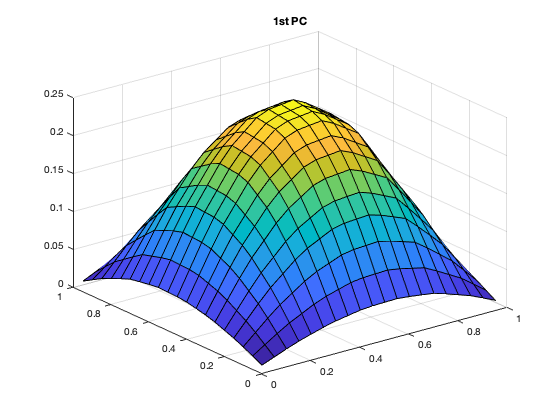
\includegraphics{../figures/pc1-surf.png}

}

\caption{\label{fig-pc1-surf}First principal component of the 8x8
B-Splines on evenly distributed locations}

\end{figure}%

\begin{figure}

\centering{

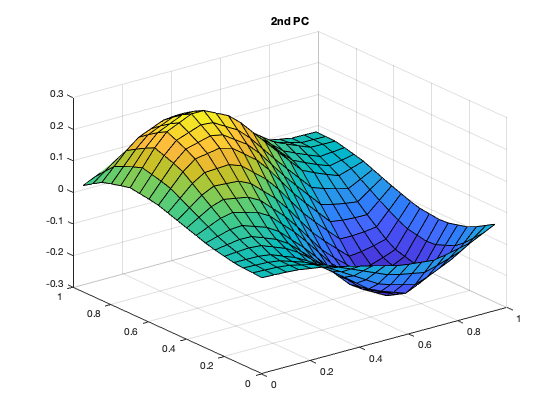
\includegraphics{../figures/pc2-surf.png}

}

\caption{\label{fig-pc2-surf}Second principal component of the 8x8
B-Splines on evenly distributed locations}

\end{figure}%

\begin{figure}

\centering{

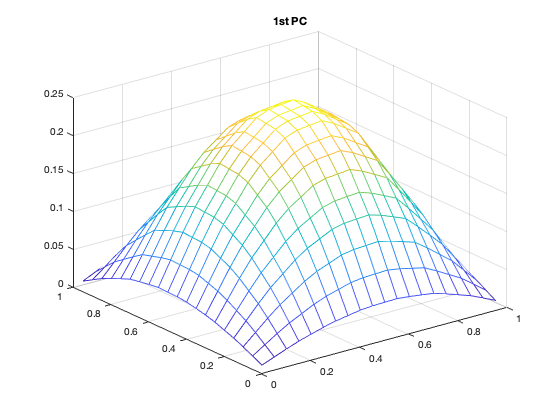
\includegraphics{../figures/pc1-mesh.png}

}

\caption{\label{fig-pc1-mesh}First principal component of the 8x8
B-Splines on evenly distributed locations}

\end{figure}%

\begin{figure}

\centering{

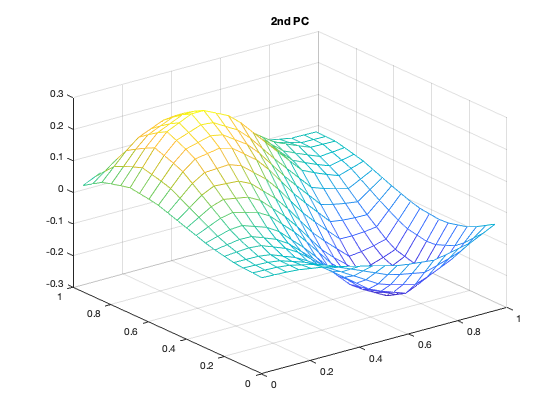
\includegraphics{../figures/pc2-mesh.png}

}

\caption{\label{fig-pc2-mesh}Second principal component of the 8x8
B-Splines on evenly distributed locations}

\end{figure}%

\begin{table}

\caption{\label{tbl-pc-NN0}Rejection frequencies testing the null
hypothesis that the slope is statically different from the true value,
zero, at the 5\% significance level for different values of spatial
correlation (\(\rho\)), using the \textbf{Gaussian} kernel HAC variance
estimator for the standard error for different cutoff lengths. The table
compares estimates of pre-whitening by including the number of principal
components of the \textbf{8x8} \textbf{triangle} B-splines that
minimizes the nearest neighbor correlation to 0\%. 1000 simulations. 500
points. Column \emph{Corr} shows the theoretical correlation at distance
\(h=0.1\), \(Corr=\rho*\exp(-\frac{1}{\sqrt{2}})\). Cutoff lengths are
equal to \(2\sigma\) in the Gaussian kernel. NN is the nearest neighbor
correlation after pre-whitening with the B-Splines. PCs is the average
number of principal components used in simulations.}

\centering{

\begin{tabular}{rrrrrrrrrrrr}
\toprule
\multicolumn{2}{c}{ } & \multicolumn{4}{c}{No Splines} & \multicolumn{6}{c}{Triangle Splines} \\
\cmidrule(l{3pt}r{3pt}){3-6} \cmidrule(l{3pt}r{3pt}){7-12}
\multicolumn{2}{c}{ } & \multicolumn{3}{c}{HAC} & \multicolumn{1}{c}{ } & \multicolumn{3}{c}{HAC} \\
\cmidrule(l{3pt}r{3pt}){3-5} \cmidrule(l{3pt}r{3pt}){7-9}
$\rho$ & Corr & .05 & .10 & .15 & HR & .05 & .10 & .15 & HR  & NN & PCs\\
\midrule
0.0 & 0.00 & 0.06 & 0.06 & 0.06 & 0.06 & 0.06 & 0.06 & 0.06 & 0.06 & -0.02 & 11.64\\
0.1 & 0.05 & 0.07 & 0.07 & 0.07 & 0.08 & 0.06 & 0.05 & 0.06 & 0.06 & 0.00 & 21.10\\
0.2 & 0.10 & 0.13 & 0.12 & 0.11 & 0.14 & 0.07 & 0.07 & 0.07 & 0.07 & 0.00 & 31.39\\
0.3 & 0.15 & 0.16 & 0.13 & 0.12 & 0.18 & 0.05 & 0.05 & 0.05 & 0.05 & 0.00 & 39.07\\
0.4 & 0.20 & 0.24 & 0.19 & 0.16 & 0.27 & 0.06 & 0.05 & 0.06 & 0.06 & 0.01 & 46.61\\
\addlinespace
0.5 & 0.25 & 0.26 & 0.21 & 0.16 & 0.32 & 0.06 & 0.06 & 0.06 & 0.06 & 0.01 & 54.73\\
0.6 & 0.30 & 0.30 & 0.22 & 0.17 & 0.37 & 0.07 & 0.06 & 0.06 & 0.07 & 0.02 & 59.83\\
0.7 & 0.35 & 0.37 & 0.28 & 0.22 & 0.48 & 0.07 & 0.07 & 0.07 & 0.08 & 0.04 & 62.51\\
0.8 & 0.39 & 0.39 & 0.28 & 0.23 & 0.52 & 0.09 & 0.07 & 0.07 & 0.09 & 0.06 & 63.14\\
0.9 & 0.44 & 0.43 & 0.31 & 0.24 & 0.57 & 0.09 & 0.08 & 0.07 & 0.11 & 0.08 & 63.16\\
\addlinespace
1.0 & 0.49 & 0.42 & 0.30 & 0.22 & 0.59 & 0.13 & 0.11 & 0.10 & 0.18 & 0.10 & 63.32\\
\bottomrule
\end{tabular}

}

\end{table}%

\begin{table}

\caption{\label{tbl-pc-ci-NN0}Confidence Interval length of different
HAC variance estimators for the standard error with the number of
principal components of the \textbf{8x8} \textbf{triangular} B-splines
that minimize the residuals' nearest neighbor correlation to 0\%. 1000
simulations. \textbf{500} points. Column \emph{Corr} shows the
theoretical correlation at distance \(h=0.1\),
\(corr=\rho*\exp(-\frac{1}{\sqrt{2}})\).}

\centering{

\begin{tabular}{rrrrrr}
\toprule
\multicolumn{2}{c}{ } & \multicolumn{3}{c}{HAC} \\
\cmidrule(l{3pt}r{3pt}){3-5}
$\rho$ & Corr & .05 & .10 & .15 & HR\\
\midrule
0.0 & 0.00 & 0.18 & 0.18 & 0.17 & 0.17\\
0.1 & 0.05 & 0.18 & 0.18 & 0.18 & 0.17\\
0.2 & 0.10 & 0.18 & 0.18 & 0.18 & 0.18\\
0.3 & 0.15 & 0.18 & 0.18 & 0.18 & 0.18\\
0.4 & 0.20 & 0.18 & 0.19 & 0.19 & 0.17\\
\addlinespace
0.5 & 0.25 & 0.19 & 0.19 & 0.19 & 0.17\\
0.6 & 0.30 & 0.19 & 0.19 & 0.19 & 0.17\\
0.7 & 0.35 & 0.19 & 0.19 & 0.20 & 0.17\\
0.8 & 0.39 & 0.19 & 0.20 & 0.20 & 0.17\\
0.9 & 0.44 & 0.20 & 0.21 & 0.22 & 0.17\\
\addlinespace
1.0 & 0.49 & 0.22 & 0.23 & 0.24 & 0.17\\
\bottomrule
\end{tabular}

}

\end{table}%

\begin{figure}[H]

{\centering 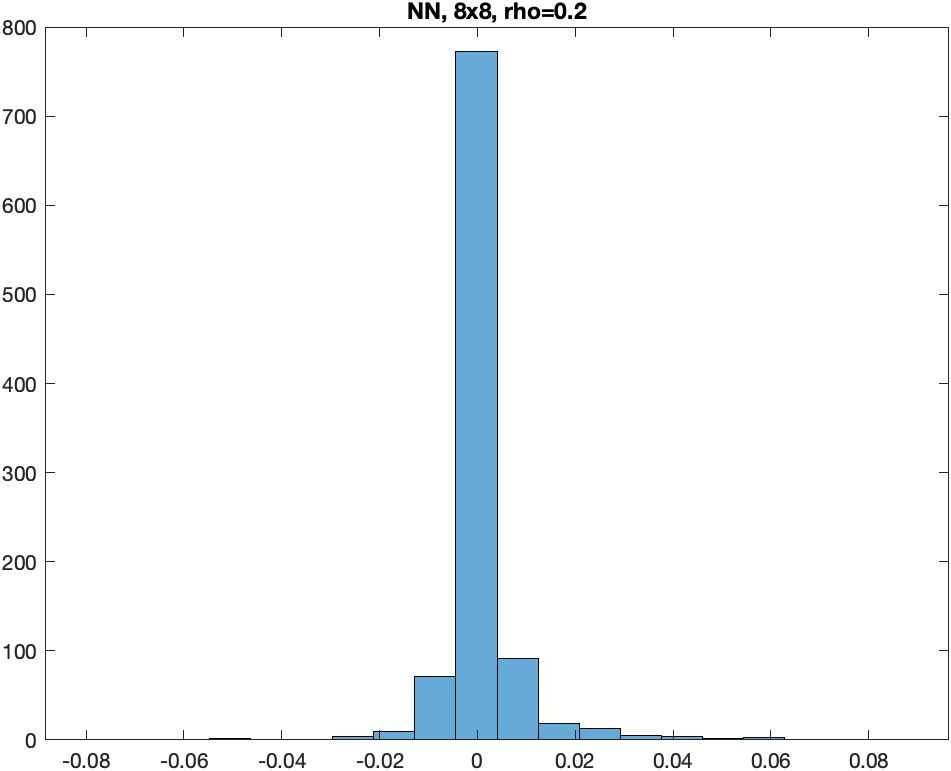
\includegraphics{../figures/hist_nn_rho-0.2_Opt_PC_NN_0.png}

}

\caption{Histogram of NN Correlation during simulations; 1000 sims; 8x8
BSplines;\(\rho=0.2\)}

\end{figure}%%
\begin{figure}[H]

{\centering 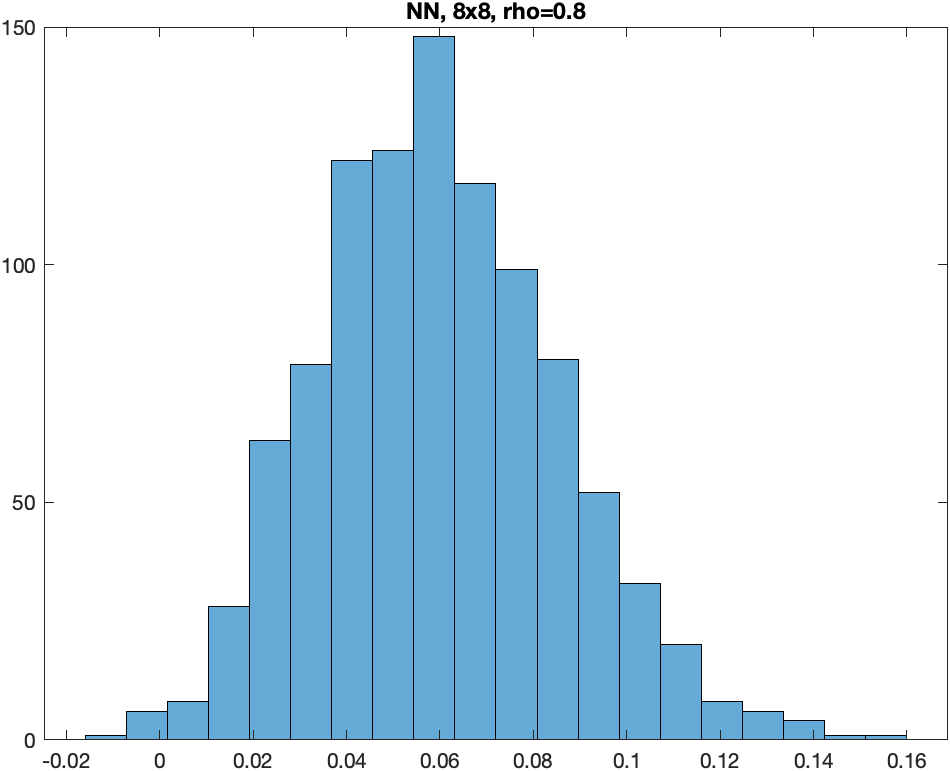
\includegraphics{../figures/hist_nn_rho-0.8_Opt_PC_NN_0.png}

}

\caption{Histogram of NN Correlation during simulations; 1000 sims; 8x8
BSplines;\(\rho=0.8\)}

\end{figure}%

\begin{table}

\caption{\label{tbl-pc-NN0-10x10}Rejection frequencies testing the null
hypothesis that the slope is statically different from the true value,
zero, at the 5\% significance level for different values of spatial
correlation (\(\rho\)), using the \textbf{Gaussian} kernel HAC variance
estimator for the standard error for different cutoff lengths. The table
compares estimates of pre-whitening by including the number of principal
components of the \textbf{10x10} \textbf{triangle} B-splines that
minimizes the nearest neighbor correlation to 0\%. 1000 simulations. 500
points. Column \emph{Corr} shows the theoretical correlation at distance
\(h=0.1\), \(Corr=\rho*\exp(-\frac{1}{\sqrt{2}})\). Cutoff lengths are
equal to \(2\sigma\) in the Gaussian kernel. NN is the nearest neighbor
correlation after pre-whitening with the B-Splines. PCs is the average
number of principal components used in simulations.}

\centering{

\begin{tabular}{rrrrrrrrrrrr}
\toprule
\multicolumn{2}{c}{ } & \multicolumn{4}{c}{No Splines} & \multicolumn{6}{c}{Triangle Splines} \\
\cmidrule(l{3pt}r{3pt}){3-6} \cmidrule(l{3pt}r{3pt}){7-12}
\multicolumn{2}{c}{ } & \multicolumn{3}{c}{HAC} & \multicolumn{1}{c}{ } & \multicolumn{3}{c}{HAC} \\
\cmidrule(l{3pt}r{3pt}){3-5} \cmidrule(l{3pt}r{3pt}){7-9}
$\rho$ & Corr & .05 & .10 & .15 & HR & .05 & .10 & .15 & HR  & NN & PCs\\
\midrule
0.0 & 0.00 & 0.06 & 0.06 & 0.06 & 0.06 & 0.06 & 0.06 & 0.06 & 0.06 & -0.02 & 11.55\\
0.1 & 0.05 & 0.07 & 0.07 & 0.07 & 0.08 & 0.05 & 0.05 & 0.06 & 0.05 & 0.00 & 21.52\\
0.2 & 0.10 & 0.13 & 0.12 & 0.11 & 0.14 & 0.07 & 0.07 & 0.07 & 0.07 & 0.00 & 32.58\\
0.3 & 0.15 & 0.16 & 0.13 & 0.12 & 0.18 & 0.05 & 0.05 & 0.06 & 0.05 & 0.00 & 40.02\\
0.4 & 0.20 & 0.24 & 0.19 & 0.16 & 0.27 & 0.06 & 0.06 & 0.06 & 0.06 & 0.00 & 48.72\\
\addlinespace
0.5 & 0.25 & 0.26 & 0.21 & 0.16 & 0.32 & 0.05 & 0.05 & 0.06 & 0.06 & 0.00 & 60.26\\
0.6 & 0.30 & 0.30 & 0.22 & 0.17 & 0.37 & 0.06 & 0.06 & 0.06 & 0.06 & 0.00 & 70.48\\
0.7 & 0.35 & 0.37 & 0.28 & 0.22 & 0.48 & 0.07 & 0.07 & 0.07 & 0.08 & 0.01 & 82.56\\
0.8 & 0.39 & 0.39 & 0.28 & 0.23 & 0.52 & 0.06 & 0.06 & 0.06 & 0.06 & 0.01 & 93.45\\
0.9 & 0.44 & 0.43 & 0.31 & 0.24 & 0.57 & 0.09 & 0.07 & 0.06 & 0.10 & 0.03 & 97.29\\
\addlinespace
1.0 & 0.49 & 0.42 & 0.30 & 0.22 & 0.59 & 0.11 & 0.10 & 0.09 & 0.15 & 0.05 & 97.69\\
\bottomrule
\end{tabular}

}

\end{table}%

\begin{table}

\caption{\label{tbl-pc-ci-NN0-10x10}Confidence Interval length of
different HAC variance estimators for the standard error with the number
of principal components of the \textbf{10x10} \textbf{triangular}
B-splines that minimize the residuals' nearest neighbor correlation to
0\%. 1000 simulations. \textbf{500} points. Column \emph{Corr} shows the
theoretical correlation at distance \(h=0.1\),
\(corr=\rho*\exp(-\frac{1}{\sqrt{2}})\).}

\centering{

\begin{tabular}{rrrrrr}
\toprule
\multicolumn{2}{c}{ } & \multicolumn{3}{c}{HAC} \\
\cmidrule(l{3pt}r{3pt}){3-5}
$\rho$ & Corr & .05 & .10 & .15 & HR\\
\midrule
0.0 & 0.00 & 0.18 & 0.18 & 0.17 & 0.17\\
0.1 & 0.05 & 0.18 & 0.18 & 0.18 & 0.17\\
0.2 & 0.10 & 0.18 & 0.18 & 0.18 & 0.18\\
0.3 & 0.15 & 0.18 & 0.18 & 0.18 & 0.18\\
0.4 & 0.20 & 0.19 & 0.19 & 0.19 & 0.17\\
\addlinespace
0.5 & 0.25 & 0.19 & 0.19 & 0.19 & 0.17\\
0.6 & 0.30 & 0.19 & 0.19 & 0.20 & 0.17\\
0.7 & 0.35 & 0.20 & 0.20 & 0.20 & 0.17\\
0.8 & 0.39 & 0.20 & 0.21 & 0.21 & 0.17\\
0.9 & 0.44 & 0.21 & 0.21 & 0.22 & 0.17\\
\addlinespace
1.0 & 0.49 & 0.22 & 0.23 & 0.24 & 0.17\\
\bottomrule
\end{tabular}

}

\end{table}%

\begin{figure}[H]

{\centering 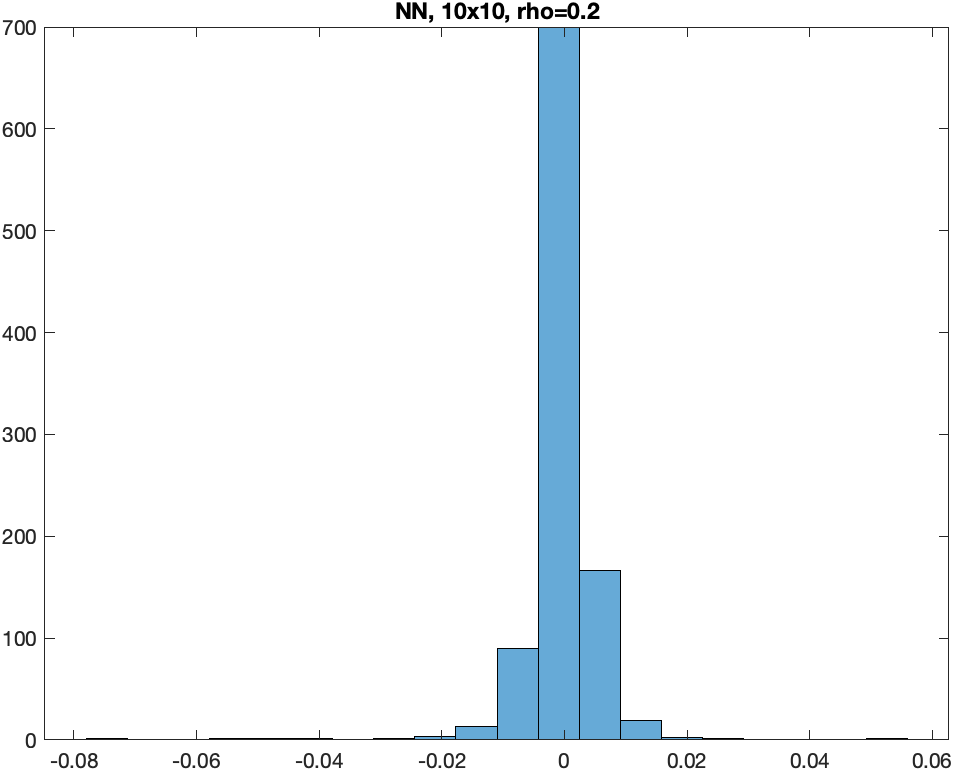
\includegraphics{../figures/hist_nn_rho-0.2_Opt_PC_NN_0_10x10.png}

}

\caption{Histogram of NN Correlation during simulations; 1000 sims;
10x10 BSplines;\(\rho=0.2\)}

\end{figure}%%
\begin{figure}[H]

{\centering 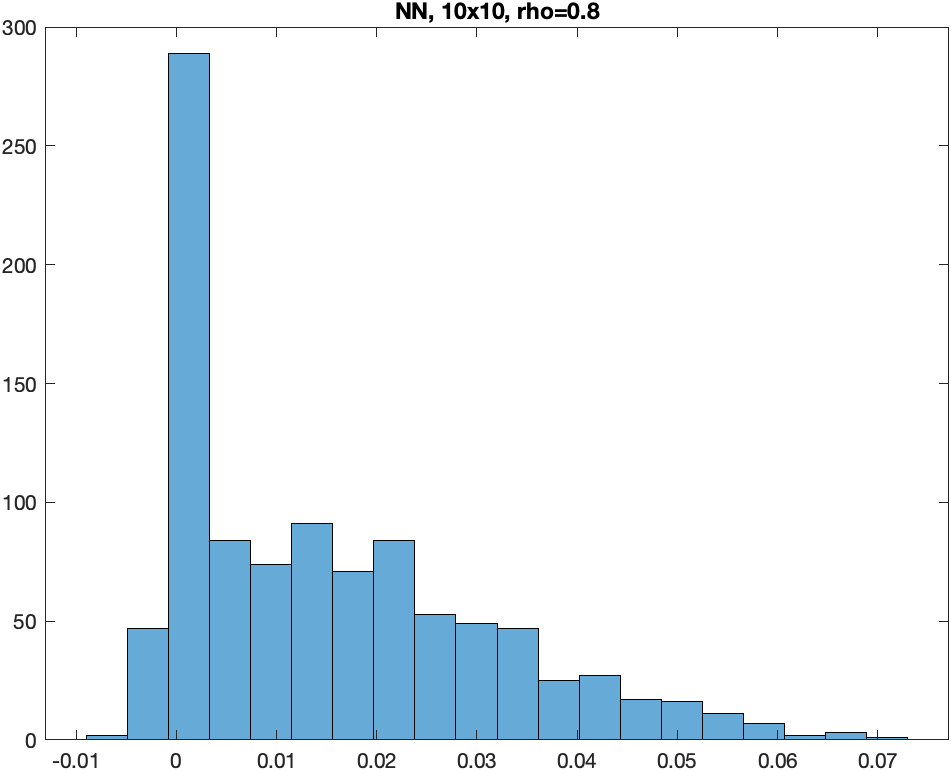
\includegraphics{../figures/hist_nn_rho-0.8_Opt_PC_NN_0_10x10.png}

}

\caption{Histogram of NN Correlation during simulations; 1000 sims;
10x10 BSplines;\(\rho=0.8\)}

\end{figure}%



\end{document}
